\documentclass[12pt,letterpaper]{article}
\usepackage{fullpage}
\usepackage[top=2cm, bottom=4.5cm, left=2.5cm, right=2.5cm]{geometry}
\usepackage{amsmath,amsthm,amsfonts,amssymb,amscd}
\usepackage{lastpage}
\usepackage{enumerate}
\usepackage{fancyhdr}
\usepackage{mathrsfs}
\usepackage{xcolor}
\usepackage{graphicx}
\usepackage{listings}
\usepackage{hyperref}

\hypersetup{%
  colorlinks=true,
  linkcolor=blue,
  linkbordercolor={0 0 1}
}

\renewcommand\lstlistingname{Algorithm}
\renewcommand\lstlistlistingname{Algorithms}
\def\lstlistingautorefname{Alg.}

\lstdefinestyle{Python}{
    language        = Python,
    frame           = lines,
    basicstyle      = \footnotesize,
    keywordstyle    = \color{blue},
    stringstyle     = \color{green},
    commentstyle    = \color{red}\ttfamily
}

\lstdefinestyle{Bash}{
   basicstyle=\footnotesize,
   stringstyle=\color{red},
   keywordstyle=\color{blue},
   commentstyle=\color{darkgrey}\slshape,
   morekeywords={linestyle,linetype,linewidth,linecolor,pointtype,nohidden3d,hidden3d,palette,lt,lw,lc,pt,ps,fd,fill,fs,ls},
   framexleftmargin=1mm, framextopmargin=1mm, frame=single
 }

 \lstdefinestyle{BBash}{
   backgroundcolor=\color{lightgray},
   basicstyle=\footnotesize,
   stringstyle=\color{red},
   keywordstyle=\color{blue},
   commentstyle=\color{darkgrey}\slshape,
   morekeywords={linestyle,linetype,linewidth,linecolor,pointtype,nohidden3d,hidden3d,palette,lt,lw,lc,pt,ps,fd,fill,fs,ls},
   framexleftmargin=1mm, framextopmargin=1mm, frame=single
 }

\lstdefinestyle{C++}{
    language        = C++,
    frame           = lines,
    basicstyle      = \footnotesize,
    keywordstyle    = \color{blue},
    stringstyle     = \color{green},
    commentstyle    = \color{red}\ttfamily
}

\setlength{\parindent}{0.0in}
\setlength{\parskip}{0.05in}

\pagestyle{fancyplain}
\headheight 35pt

\chead{\textbf{\Large ExaHyPE 2 Training}}
\rhead{ \today}
\lfoot{}
\cfoot{}
\rfoot{\small\thepage}
\headsep 1.5em

\begin{document}

\begin{figure}[!h]
\centering

\includegraphics[width=0.75\linewidth]{ExaHyPE_Logo.jpg}
\end{figure}

\section{Introduction}
\label{sec:Introduction}

\vspace{0.2cm}

This will be a brief introduction into ExaHyPE 2. ExaHyPE 2 is a hyperbolic PDE engine, this means it solves PDEs which have a finite propagation speed,
like those representing sound, elastic waves or magnetism. That's anything of the following form:\\

\begin{equation*}\label{ExaHyPE2_formulation}
    \frac{\partial Q}{\partial t} + \nabla . F(Q, \nabla Q) + B(Q) . \nabla Q= S(Q) + \sum_{i = 1}^{n_{ps}} \delta_i
\end{equation*}
\\

The goal of ExaHyPE 2 is to make it easy for users to run optimized code without needing an
entire computer science degree. We provide (via the parent project Peano 4) single-core or multi-core parallelization,
GPU offloading, multiple PDE solvers, storage optimizations, dynamic adaptive mesh refinement and load balancing and so on.
The user then only needs to specify which optimizations they want, and implement the specifics of their hyperbolic PDEs.\\

Let's move on and see what that looks like, shall we? \\

\newpage

\section{Getting Your Peano Installation}
\label{section_2}
If you haven't already downloaded our training Docker file, or if you don't have Docker installed, now would be a great time to do that.

Follow the Docker installation guide for your operating system (\url{https://docs.docker.com/engine/install/}) and run Docker.

You can simply pull the prebuilt Docker image containing an ExaHyPE 2 and a Peano 4 installation by

\begin{lstlisting}[style = Bash]
docker pull peanoframework/training
\end{lstlisting}

Now that this is done, you should have a working installation of Peano, so let's go give it a spin!

After installation, run

\begin{lstlisting}[style = Bash]
docker run --rm -p 9999:9999 peanoframework/training
\end{lstlisting}

You should see

\begin{lstlisting}[style = Bash]
http://127.0.0.1:9999/lab?token=
\end{lstlisting}

Click on that link (ctrl+left-click) or enter the link in the address bar of your web browser.

You can also run an interactive Docker container and mount the training repository:

\begin{lstlisting}[style = Bash]
docker run -it -v ${PWD}:/training --rm -p 9999:9999 peanoframework/training
\end{lstlisting}

Then you may start the jupyter lab session in the `/training` folder:

\begin{lstlisting}[style = Bash]
jupyter lab --allow-root --port=9999 --no-browser --ip=0.0.0.0
\end{lstlisting}

\newpage

\section{Our First Configuration File}
\label{section_3}

We have Peano 4 and ExaHyPE 2 installed, but how do we use it? For this, let's take a look at our first configuration file, in \textbf{Acoustic/PlanarWaves.py}\\
The configuration files are in \texttt{Python}, so it should surprise no one that they start with the following:\\

\begin{lstlisting}[style = Python]
import peano4, exahype2
\end{lstlisting}

With our imports out of the way, we are free to define our problem, for this, let's start with a solver:\\

\begin{lstlisting}[style = Python]
my_solver = exahype2.solvers.aderdg.rusanov.GlobalAdaptiveTimeStep(
    name                  = "PlanarAcousticSolver",
    order                 = 5,
    min_cell_h            = 0.1,
    max_cell_h            = 0.1,
    time_step_relaxation  = 0.9,
    unknowns              = {"p": 1, "v": 2},
    auxiliary_variables   = {}
)
\end{lstlisting}

This creates an \textit{ADER-DG} solver of discretization order 5 named \textbf{PlanarAcousticSolver} with adaptive timestepping and two unknowns:
\textbf{p} and \textbf{v}, with \textbf{v} having a multiplicity of two (i.e., we have two velocities).
Unknowns and auxiliary variables can be either specified by indicating how many there are (\texttt{unknowns = 3}),
in which case users must keep track of them manually, or they can be specified via a dictionary, which will allow us to access them by name.\\

Now that we have a solver, let's define the problem we want to solve, and while we're at it let's add a simple optimization:\\

\begin{lstlisting}[style = Python]
my_solver.set_implementation(
    flux = exahype2.solvers.PDETerms.User_Defined_Implementation
)

my_solver.add_kernel_optimizations(is_linear=True)
\end{lstlisting}

This is again relatively self-explanatory: The acoustic equations do not require sources or a non-conservative flux,
so the only term from equation \ref{ExaHyPE2_formulation} that remains is the flux.
\texttt{exahype2.solvers.PDETerms.User\_Defined\_Implementation} means we want to define this manually.\\
With this out of the way, we need to create an environment for the solver to run in, this is a \textbf{ExaHyPE 2} project:\\

\begin{lstlisting}[style = Python]
my_project = exahype2.Project(
    namespace     = ["exahype2", "training", "acoustic"],
    directory     = ".",
    project_name  = "PlanarWaves",
    executable    = "PlanarWaves"
)

my_project.add_solver(my_solver)
\end{lstlisting}

This handles things like the grid generation, traversal, data exchanges and such.
Once again we need to populated it with some data, such as the number of dimensions our problem is in,
the size of the domain, how long the simulation should run for and when to plot.\\

We can also specify here whether we want to use periodic boundary conditions:\\

\begin{lstlisting}[style = Python]
my_project.set_global_simulation_parameters(
    dimensions            = 2,
    size                  = [2.0,  2.0],
    offset                = [-1.0, -1.0],
    min_end_time          = 1.414,  # sqrt(2)
    max_end_time          = 1.414,  # sqrt(2)
    first_plot_time_stamp = 0.0,
    time_in_between_plots = 0.1,
    periodic_BC           = [True, True],
)
\end{lstlisting}

Finally, we have some more optimizations for the project, and then we can generate all the glue code we need and compile it:\\

\begin{lstlisting}[style = Python]
my_project.set_load_balancing(
    "toolbox::loadbalancing::strategies::SpreadOutOnceGridStagnates",
    "new ::exahype2::LoadBalancingConfiguration()"
)

my_project.set_Peano4_installation("../../", peano4.output.CompileMode.Release)

my_project = my_project.generate_Peano4_project()
my_project.build(make=True, make_clean_first=True)
\end{lstlisting}

Once this is finished compiling, let's run it:\\

\begin{lstlisting}[style = Bash]
./PlanarWaves
\end{lstlisting}

And, while this is running, let's go take a look at our implementation so we can actually figure out what we're simulating!

\newpage

\section{Our First Implementation File}
The astute reader might have noticed that before we built our project, there was one other file already present within the same directory: \textbf{PlanarAcousticSolver.cpp}.
We will be taking a look at this file next since, as you most likely have already guessed, it contains the implementation of our PDE.
\\ \\
Before we do this however, we will quickly define the PDE that is to come. As the name of the file will have already indicated,
this is the two-dimensional acoustic equation which appears as follows:

\begin{equation*} \label{Acoustic_equation}
    \frac{\partial}{\partial t}\left(
    \begin{array}{lr} p \\
                      v_1 \\
                      v_2
                      \end{array} \right) +
    \nabla \begin{pmatrix}
                      K_0 v_1          & K_0 v_2\\
                      \frac{p}{\rho}   & 0 \\
                      0                & \frac{p}{\rho}
    \end{pmatrix}  = \vec{0}
\end{equation*}

where $p$ is the pressure, and $v_1$ and $v_2$ are the velocity respectively in the $x-$ and $y-$direction.
It additionally uses two parameters which, for simplicity's sake we have assumed to remain constant over the domain.
These are the density $\rho=1$ and the bulk modulus $K_0=4$, which you can think of as the squishiness of the material (don't ask, we don't have time).\\
In order to implement this equation, we need two things: a flux, and a maximal eigenvalue.
The maximal eigenvalue is the greatest eigenvalue of the flux tensor, which is:

\begin{equation*} \label{Acoustic_eigenvalue}
    \lambda = \sqrt{\frac{K_0}{\rho}}
\end{equation*}

This is required for the Riemann-solver (again, don't ask) and the timestepping, and is implemented in the first function of our file:\\

\begin{lstlisting}[style = C++]
double ::exahype2::training::acoustic::PlanarAcousticSolver::maxEigenvalue(
  const double* __restrict__                      Q,
  const ::tarch::la::Vector<Dimensions, double>&  x,
  const ::tarch::la::Vector<Dimensions, double>&  h,
  double                                          t,
  double                                          dt,
  int                                             normal
) {
  constexpr double K0   = 4.0;
  constexpr double rho  = 1.0;
  constexpr double c    = std::sqrt(4.0 / rho);

  return c;
}
\end{lstlisting}

\newpage

Next is the flux, we have already defined it in \ref{Acoustic_equation}, so let's look at the implementation:\\

\begin{lstlisting}[style = C++]
void ::exahype2::training::acoustic::PlanarAcousticSolver::flux(
  const double* __restrict__                      Q,
  const ::tarch::la::Vector<Dimensions, double>&  x,
  const ::tarch::la::Vector<Dimensions, double>&  h,
  double                                          t,
  double                                          dt,
  int                                             normal,
  double* __restrict__                            F
) {
  constexpr double K0 = 4.0, rho = 1.0;

  switch(normal) {
    case 0: // Flux in x-direction
      F[s.p]      = K0 * Q[s.v + normal];
      F[s.v + 0]  = Q[s.p] / rho;
      F[s.v + 1]  = 0.0;
      break;
    case 1: // Flux in y-direction
      F[s.p]      = K0 * Q[s.v + normal];
      F[s.v + 0]  = 0.0;
      F[s.v + 1]  = Q[s.p] / rho;
  }
}
\end{lstlisting}

The flux has one component for each direction, which one we need is determined by the \texttt{normal}-parameter,
and it depends on the values of the equation, which are found in \texttt{Q}.\\
These two are sufficient to define the entire equation, a measly two functions and less than twenty lines of code.
But we still need to define our initial conditions, we do so in the function appropriately-named \texttt{initialCondition},
and we prescribe a sinus for the initial conditions:\\

\begin{lstlisting}[style = C++]
void ::exahype2::training::acoustic::PlanarAcousticSolver::initialCondition(
  double* __restrict__                            Q,
  const ::tarch::la::Vector<Dimensions, double>&  x,
  const ::tarch::la::Vector<Dimensions, double>&  h,
  const ::tarch::la::Vector<Dimensions, int>&     index,
  bool                                            gridIsConstructed
) {
  const double val = cos(-std::numbers::pi*(x[0] + x[1]));
  constexpr double K0 = 4.0, rho = 1.0;
  constexpr double kr = std::sqrt(2 * K0 * rho);

  Q[s.v + 0] = val;
  Q[s.v + 1] = val;
  Q[s.p]     = kr * val;
}
\end{lstlisting}

Finally, we would normally need to define boundary conditions to make our problem well-defined,
but as we have specified periodic boundary conditions, this is not necessary here.\\

So, now that we've gone through all of this, let's go take a look at our results.
These should be within the folder \texttt{solutions} and are stored in a custom format named \texttt{peano-patch-file},
which is essentially plain-text but allows for efficient parallel writing.\\
In order to visualize this, we will first need to convert these files using following command:\\

\begin{lstlisting}[style = Bash]
python $PEANO_ROOT/python/peano4/visualisation/render.py \
  solutions/solution-PlanarAcousticSolver.peano-patch-file
\end{lstlisting}

This converts the patch files them to $.vtu$ files, which we can read and visualize using e.g., ParaView:

\begin{lstlisting}[style = Bash]
paraview solutions/solution-PlanarAcousticSolver.pvd
\end{lstlisting}

If you've followed all of the steps until now, you should have following initial conditions for the pressure:

\begin{figure}[!h]
\centering
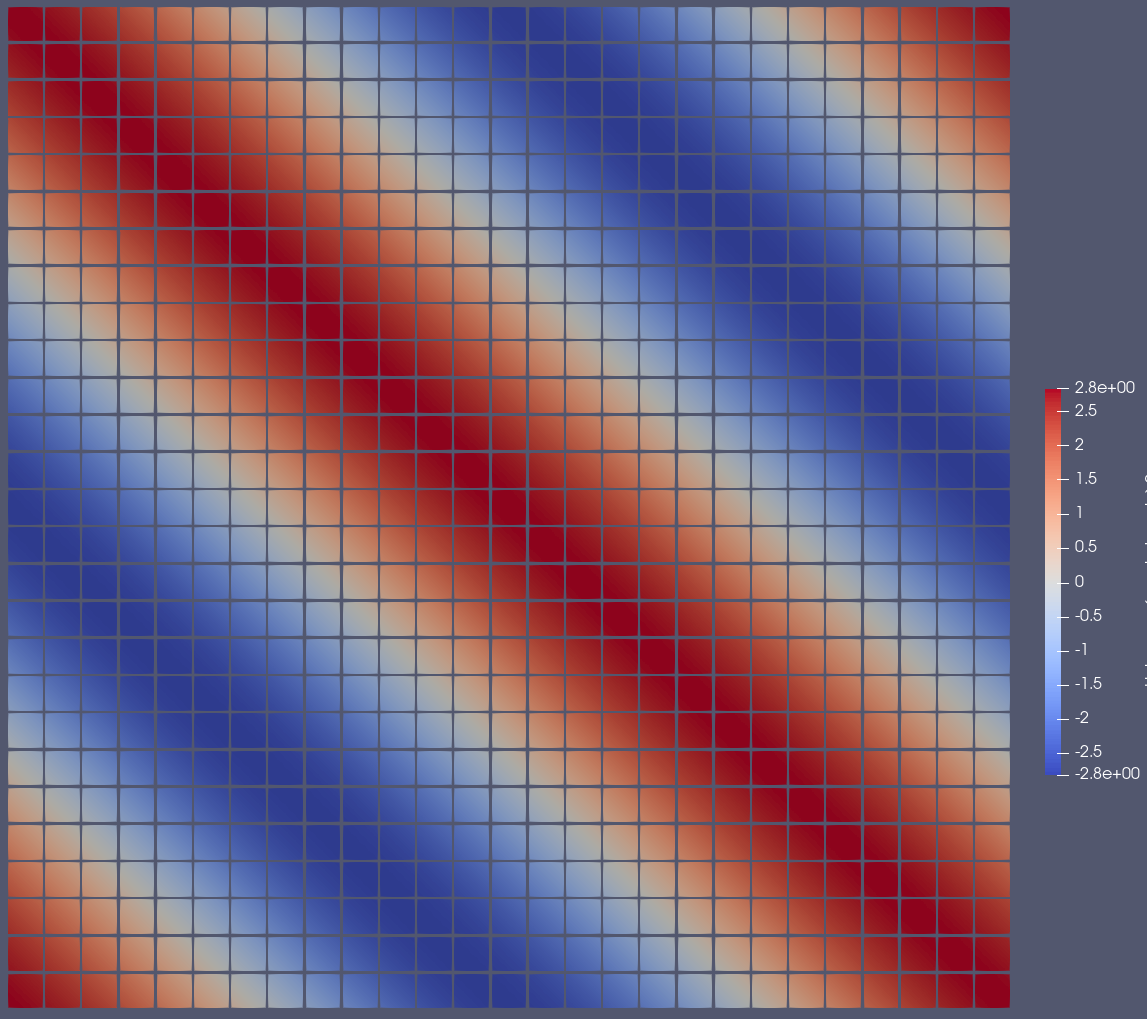
\includegraphics[width=0.60\linewidth]{PlanarAcoustic_initial.png}
\caption{The initial pressure of the acoustic equations for our scenario.}
\end{figure}

Can you tell us what these look like by the end of the simulation?

\section{Our First Exercise}
\vspace{0.2cm}

Now that we have an example of how to implement an equation,
we can try implementing our own equation, let's try out the shallow-water equations, or SWE for short:

\begin{equation*} \label{SWE_wo}
    \frac{\partial}{\partial t}\left(
    \begin{array}{lr} h \\
        h u_1 \\
        h u_2 \\
        b
        \end{array} \right) +
    \nabla \underbrace{\begin{pmatrix}
        h u_1                       & h u_2     \\
        h u_1^2 + \frac{g*h^2}{2}   & h u_1 u_2 \\
        h u_2 u_1                   & h u_2^2  + \frac{g*h^2}{2} \\
        0                           & 0
    \end{pmatrix}} = \vec{0}
\end{equation*}

With eigenvalues:

\begin{equation*}
    \left(
    \begin{array}{lr}
        \lambda_1 \\
        \lambda_2 \\
        \lambda_3
    \end{array} \right) =
    \left(
    \begin{array}{lr}
        h u_n + \sqrt{g (h+b)} \\
        h u_n \\
        h u_n - \sqrt{g (h+b)} \\
    \end{array} \right)
\end{equation*}

These are an approximation for the movement of shallow non-viscous fluids, i.e., they assume that there is no pressure
differential within the fluid, and no loss of velocity due to friction.
Their components are the water height $h$, the momentum in $x-$ and $y-$direction $hu_1$ and $hu_2$ respectively,
and the bathymetry $b$, which is the height of the ground below the liquid. They also use the gravity $g=9.81$.\\

We want to simulate a so-called \textit{dam-break scenario}, that is a scenario where a large mass of fluid spreads rapidly from an
initial resting position, such as might happen when you jump into a pool, or when you jump into a bathtub, or when you jump into a puddle. \\
A configuration file has already been created for you at \texttt{swe/dam\_break.py}.
Try running it, and then look into the generated implementation file \texttt{SWESolver.cpp}.\\

\begin{enumerate}
    \item
        First, let's implement some initial conditions. Let's start simple and set all values to $0$, except for the initial water height,
        which should be $1.0$ on the left half of the domain, and $2.0$ on the right half of the domain.
        You can access the position of the point you are at via the parameter \texttt{x}.\\
        (Hint: The size and position of your domain can be found in the configuration file.)
    \item
        Second, let's do the same thing for the boundary conditions. Here you will need to set the values outside of the domain through the
        parameter $Qoutside$, set the velocities and the bathymetry to be equal to $0$, and the water height to $1.0$ everywhere.
    \item
        Thirdly, fill out the \texttt{maxEigenvalue} function. Take care to use the proper velocity for whatever direction is being computed.\\
        (Hint: remember that the base unknowns are not $u$, but $hu$)
    \item
        Next, let's implement the flux according to \ref{SWE_wo}, in addition to this, zero out the NCP, that is to say set \texttt{BTimesDeltaQ} to $0$
        for all its components, after all we do not need an NCP here, do we?
    \item
        Once all of this is done, re-compile the project using the command \texttt{make},
        then run the executable \texttt{DamBreak} and go do some stretches while it runs.
        Maybe get a glass of water as well. Once you are finished stretching and the code is finished running,
        convert the output and visualize it, does it look like what you'd expect?
\end{enumerate}

\vspace{1cm}

\begin{figure}[!h]
\centering
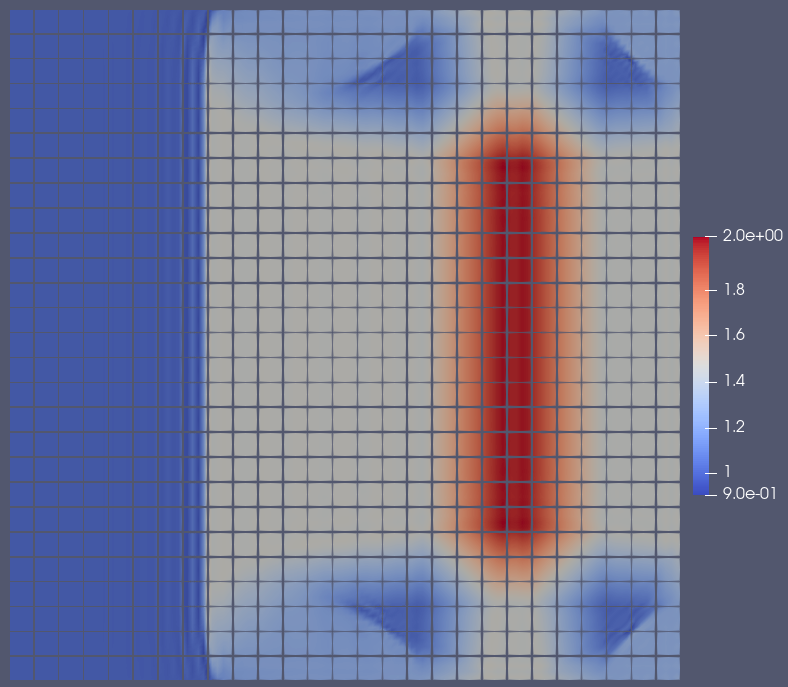
\includegraphics[width=0.70\linewidth]{SWE_wo.png}
\caption{The water height for our scenario after about 0.1s.}
\end{figure}

\newpage

\subsection{Extending SWE}

\vspace{0.2cm}

So I have to admit something. When we described the shallow-water equations to you, I sort of lied.
Well not really, it's just that \ref{SWE_wo} is the form of the SWE without bathymetry.\\
With bathymetry, it looks as follows (note that the gravity term was moved from the flux to the NCP):

\begin{equation*} \label{SWE_w}
    \frac{\partial}{\partial t}\left(
    \begin{array}{lr} h \\
        h u_1 \\
        h u_2 \\
        b 
        \end{array} \right) +
    \nabla \underbrace{\begin{pmatrix}
        h u_1           & h u_2     \\
        h u_1^2         & h u_1 u_2 \\
        h u_2 u_1       & h u_2^2   \\
        0               & 0
    \end{pmatrix}}_{ flux } +
    \underbrace{\begin{pmatrix}
        0                     & 0\\
        h g*\partial_x(b+h)   & 0\\
        0                     & h g*\partial_y(b+h) \\
        0                     & 0
    \end{pmatrix}}_{ ncp }  = \vec{0}
\end{equation*}

Let's modify our implementation to take this into account, and while we're at it change our scenario a little, and heck why not learn about mesh refinement too?\\
Mesh refinement in ExaHyPE 2 is controlled via a so-called \textit{refinement criterion}.
Cells can be sub-divided into $3^d$ cells so long as this would not cause the sub-cells to be smaller than the lowest cell size as defined in the configuration.

\begin{enumerate}
    \item
        First, let's modify our flux to remove the term that shouldn't be in it, and implement our NCP.
        The NCP is implemented into the parameter $BTimesDeltaQ$, and depends on the gradients of the values, which are stored in the parameter $deltaQ$.
    \item
        Then, let's modify our starting conditions. Let's try running a \textit{radial dam-break}, that is a circular one.
        And let's have it be dependent on the bathymetry.
        For this, set the water height to be constant at $1.0$, and the bathymetry to be $0.2$ within a distance of $0.5$ of the center of the domain,
        and $0.0$ otherwise. The velocities can remain $0$.\\
        (Hint: You can use the function \textit{::tarch::la::norm2()} to compute the norm of a vector)
    \item
        With these parameters, re-compile and re-run the simulation.
    \item
        Finally, let's try some adaptive mesh refinement. There is a function \texttt{refinementCriterion} within your implementation file which
        currently keeps the current mesh refinement no matter what.\\
        Conditionally set it to return \texttt{::exahype2::RefinementCommand::Refine} if within a distance of $0.4$ to $0.6$ of the center of the domain.\\
        With this, re-compile the project, and run it one final time.
\end{enumerate}

\newpage

\section{The Euler Equations and Air Flow Over a Symmetric Airfoil}
\label{refinement}

\vspace{0.2cm}

New exercise, new equation! This time we will be simulating the \texttt{euler equations},
which approximate the flow of non-viscous fluids, but do take into account pressure differentials.
In two dimensions, these take following form:

\begin{equation*} \label{Euler_equation}
    \frac{\partial}{\partial t}\left(
    \begin{array}{lr} \rho \\
                      \rho u_1 \\
                      \rho u_2 \\
                      E_t
                      \end{array} \right) +
    \nabla \begin{pmatrix}
                      \rho u_1          & \rho u_2\\
                      \rho u_1^2 + p    & \rho u_1 u_2 \\
                      \rho u_2 u_1      & \rho u_2^2 + p \\
                      (E_t + p) u_1     & (E_t + p) u_2
    \end{pmatrix}  = \vec{0}
\end{equation*}

The eigenvalues of the 2 dimensional euler equation are:

\begin{equation*}
    \left(
    \begin{array}{lr} \lambda_1 \\
                      \lambda_2 \\
                      \lambda_3
                      \end{array} \right) =
    \left(
    \begin{array}{lr} u - c \\
                      u \\
                      u + c
                      \end{array} \right)
\end{equation*}

We have not provided you with a configuration file, so you will need to make your own.
However since the Euler equations and the scenario we will attempt next are somewhat more unstable than the previous two (and also just to show of the features of ExaHyPE 2)
we will use a different solver. This time, we will use a \textit{Finite Volumes} solver.
This can be created in the configuration as follows:

\begin{lstlisting}[style = Python]
my_solver = exahype2.solvers.fv.rusanov.GlobalAdaptiveTimeStep(
  name                  = "EulerSolver",
  patch_size            = 22,
  min_volume_h          = min_h,
  max_volume_h          = max_h,
  time_step_relaxation  = 0.1,
  unknowns              = { "p": 0, "v": 2, "E": 1 },
  auxiliary_variables   = 0
)
\end{lstlisting}

\begin{enumerate}
    \item
        First, create and fill a configuration file. Use a Finite-Volumes solver for this, then set the domain size to $120x120$,
        the offset to $-10, -60$ and the end-time to $10.0$.
        You can choose the mesh refinement of your choice, but we recommend a depth of 5 over the whole domain.
    \item
        Once you are content with your configuration file, implement the flux and the eigenvalues for your solver.
    \item
        Next, we will set the boundary conditions. These should be $[1.0, 1.0, 0.0, 2.5, 1.0]^T$ on the leftmost face of the domain.
        On all other faces, use absorbing boundary conditions.
        That is to say the values outside of the boundary should be equal to the values inside of the boundary.
    \item
        Finally, we need to implement the initial conditions.
        We will try to simulate airflow over a symmetrical \textit{NACA airfoil}.
        Specifically we will choose airfoil \textit{NACA 0012}.
        The half-thickness of the airfoil is defined by following equation:
        \begin{equation}
            y_t = 5*0.12* ( 0.2969*\sqrt{x_n} - 0.1260*x_n - 0.3516*x_n^2 + 0.2843*x_n^3 - 0.1104*x_n^4 )
        \end{equation}
        where $x_n$ is $x/100$.
        The initial conditions within the airfoil should be $[1000, 1.0, 0.0, 2.5]^T$,
        those outside of the airfoil should be $[1.0, 1.0, 0.0, 2.5]^T$.\footnote{We have committed here what we in the business call a "not accurate cheaty fake result", there are many good ways to simulate what we want to simulate and this is not one of them. But it is easy and it'll make a nice picture if you did it right, so don't tell any of the professors in the room.}

    \item
        Compile and run! If you have done everything correctly, your initial conditions should look something like \ref{euler_initial},
        and you should see a so-called \textit{bow shock} develop over time as the flow causes higher pressure in front of your airfoil and lower pressure behind it.

    \item
        You are finished with all of the tasks we've prepared so you'll have to think up some more yourself, congratulations!
        If you'd like to feel free to experiment some more, but before that how about some more stretches?
\end{enumerate}

\begin{figure}[!h]
\centering

\includegraphics[width=0.40\linewidth]{Euler_initial.png}\label{euler_initial}
\caption{The initial condition of the Euler equations for our scenario.}
\end{figure}

\end{document}
